\labelsubsection{Results and Observations}{subsec:results_and_observations}
\todo[inline]{Observations + possible explanations}
\todo[inline]{How do the results relate to hypothesis?}
\todo[inline]{Error analysis}
\todo[inline]{Confusion matrices?}
\todo[inline]{Comparison between text n-grams and concept maps/co-occurrence graphs}
\todo[inline]{Look at concepts used in concept maps: frequency in whole corpus, ...}

\subsubsection{Structure Of The Used Graphs}
The co-occurrence graphs have a relatively simple structure.
Co-occurrence graphs are always connected, ie. the number of connected components is 1 (or 0 in case of an empty graph).
When the window size is 1, the graph is similar to a path, meaning that most of the nodes have a degree $< 2$. With increasing window size, the graph gets more connected.


\begin{figure}[ht]
\centering
\missingfigure[figcolor=white]{}
\caption{Percentage of graphs with more than one connected component. Per dataset for both concept maps and co-occurrence maps}
\end{figure}

\begin{figure}[ht]
\centering
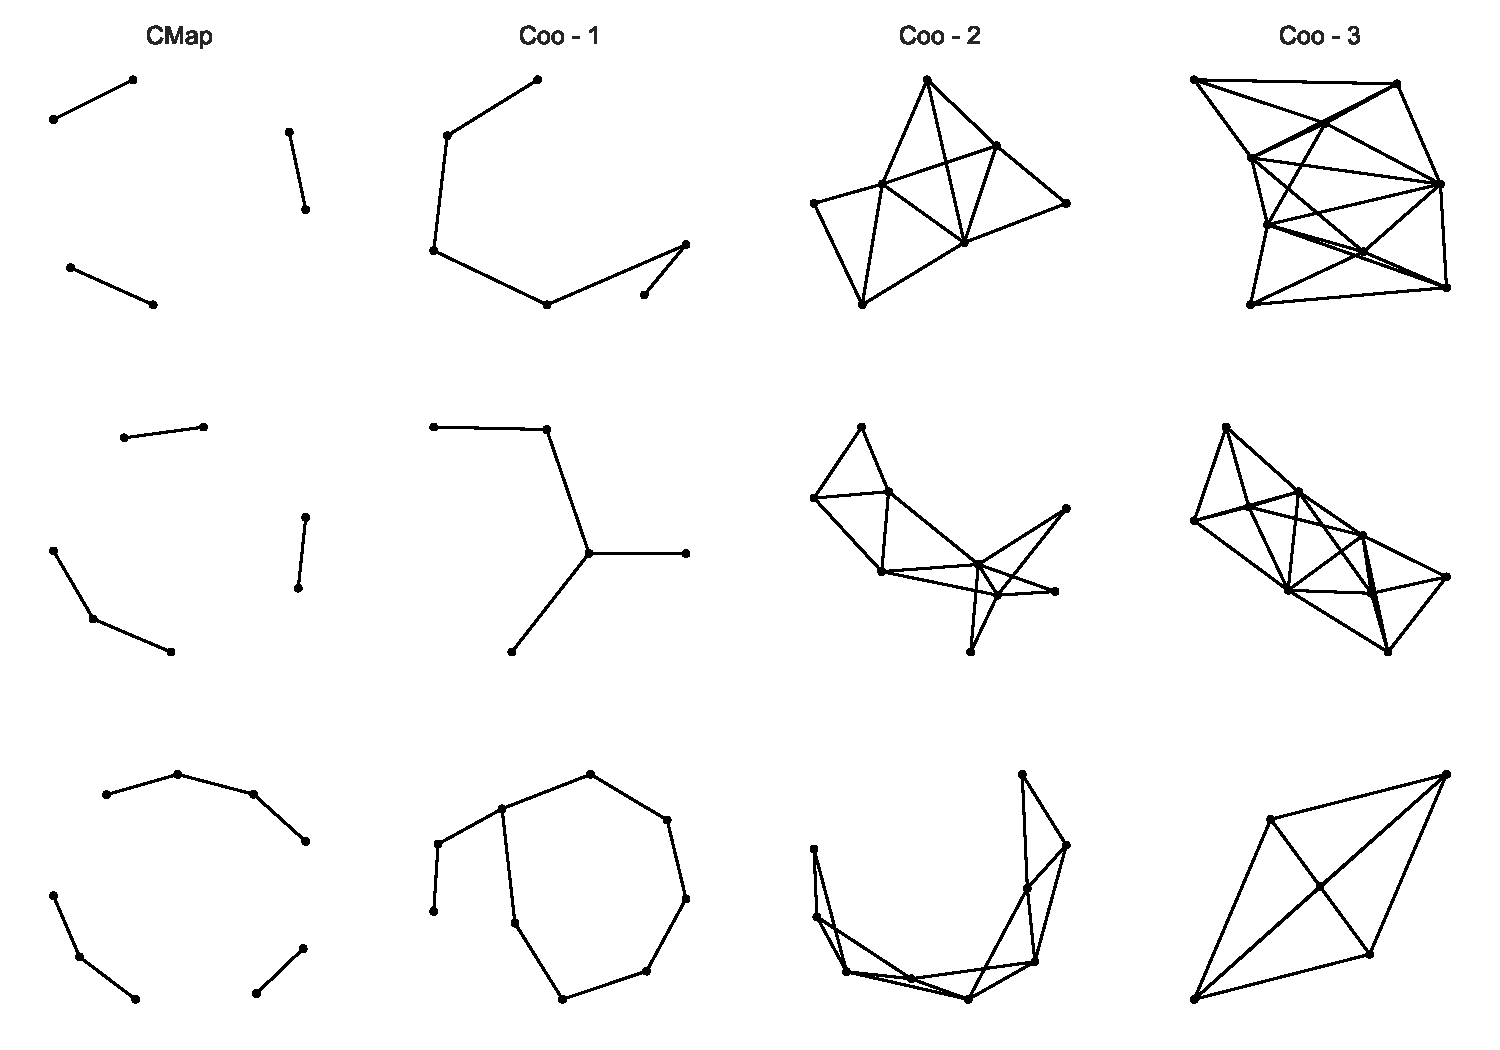
\includegraphics[width=0.6\linewidth]{assets/figures/graph-examples.pdf}
\caption{Graph examples per type. Three examples are shown per type. The concept map examples all have more than one connected component, while the co-occurrence graphs all have only one. Dataset: ling-spam}
\end{figure}

\begin{figure}[ht]
\centering
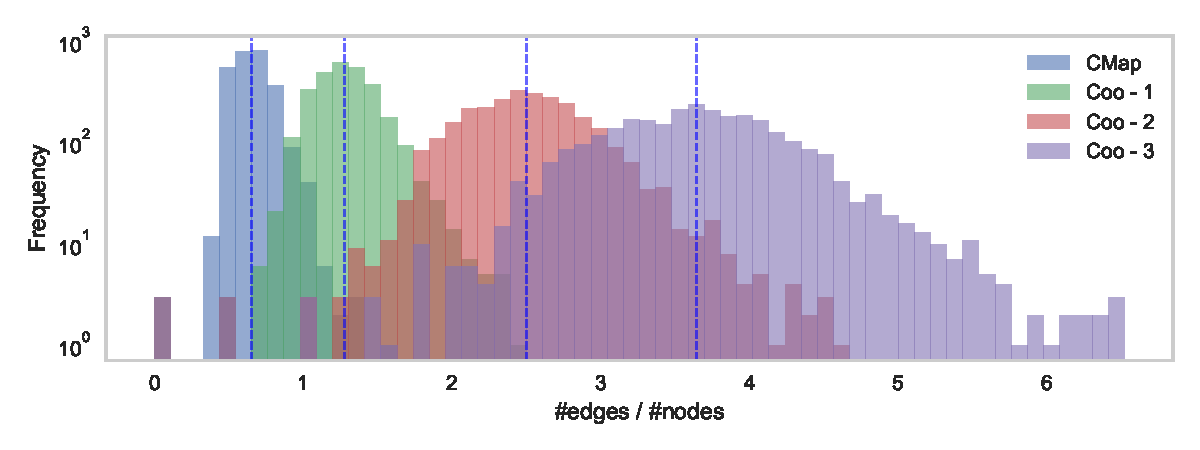
\includegraphics[width=0.7\linewidth]{assets/figures/hist-edgesnodes.pdf}
\caption{Histogram of the number of edges divided by the number of nodes. Per graph type. The lines correspond to the median value.}
\label{fig:histogram-edges-div-nodes-per-type}
\end{figure}

\begin{figure}[ht]
\centering
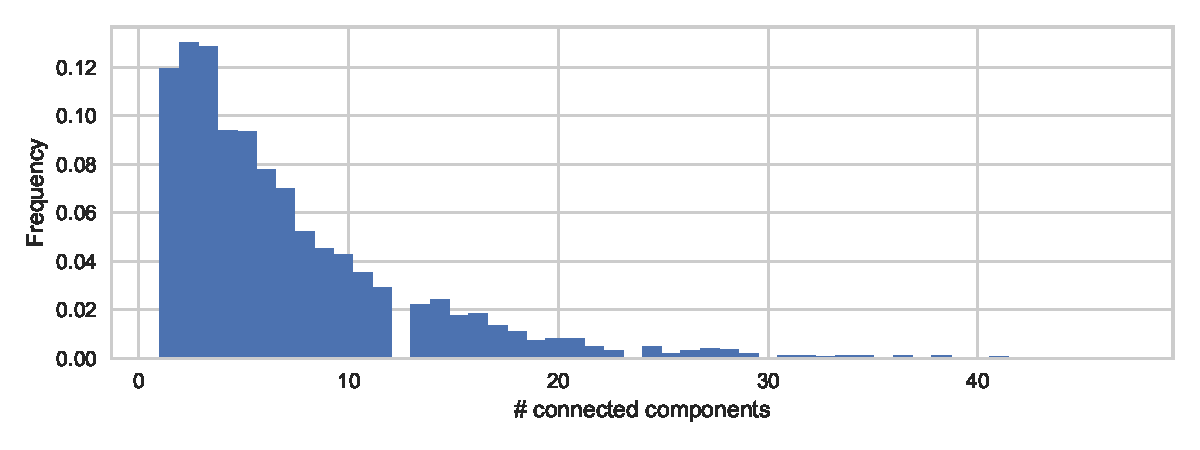
\includegraphics[width=0.8\linewidth]{assets/figures/hist-connected-components-ling-spam-CMap.pdf}
\caption{Histogram of connected components per concept map. Dataset: ling-spam.}
\end{figure}


\labelsubsection{Related And Intermediate Observations}{subsec:related_and_intermediate_observation}
\todo[inline]{Sparsity of feature vectors}
\todo[inline]{Complexity of approach}